\section{СБОР ДАННЫХ И СОЗДАНИЕ ДИАЛОГОВОЙ ЧАСТИ НАБОРА ДАННЫХ}
\subsection{СТРУКТУРА НАБОРА ДАННЫХ}
Чтобы создать набор данных для обучения диалоговой модели, которая эмулирует поведение NPC по заданному описанию в играх, необходимо иметь диалоги, построенные по определенной системе правил. Одной из самой распостраненной, обширной и гибкой системой правил, по которым можно описать NPC, является система Dungeon \& Dragons (далее D\&D), т.к. она обладает вполне определенной структурой. Например, персонажи обязаны иметь конкретное мировозрение, определяющее их поведение и взгляды на поступки, мотивацию, внешнее описание и слабости. Поэтому выбор такой системы выглядит естественным. 

Набор данных, созданный из данных игр во вселенной D\&D, должен содержать примеры диалогов NPC с главным героем и примеры описания NPC в формате Name/Alignment/Description/Flaw/Motivation/Personality.

\subsection{СБОР ДАННЫХ}
\subsubsection{СБОР И ПРЕДОБРАБОТКА ПЕРВОНАЧАЛЬНЫХ ДАННЫХ}
Первоначальные данные были получены из следующих игр: 
\begin{enumerate}
      \item <<Icewind Dale: Enhanced Edition>>.
      \item <<Planescape: Torment: Enhanced Edition>>.
\end{enumerate}

Такой выбор игр неслучаен: все эти игры были созданы с помощью  игрового движка Infinity Engine. Диалоги были получены следующим образом:
\begin{enumerate}
      \item Диалоги, которые были использованы, находились в скомпилированом файле, который можно было найти внутри <<.bif>> файла.
      \item Чтобы получить диалоги NPC в скомпилированном формате с расширением <<.dlg>>, была использована программа WinBif.
      \item Далее, с помощью WeiDU \cite{weidu-repo}, специального транслятора,
            написанного для создания собственных диалогов в играх Infinity Engine в качестве модификации, эти файлы были преобразованы в формат языка <<.d>>;.
      \item Наконец, полученные файлы конвертированы в удобный для анализа JSON-формат. Такие файлы содержат возможные диалоги NLP с главным героем.
\end{enumerate}

\subsubsection{ПОСТОБРАБОТКА ПЕРВОНАЧАЛЬНЫХ ДАННЫХ}

Для начала полученные JSON файлы были проанализированы на предмет NPC, т.к. в этих играх есть описания взаимодействия с неодушевленными предметами: порталами, сферами и т.д. Из-за того, что такие описания не содержат непосредственно диалогов, они были удалены из выборки. Также было замечено, что в игре <<Planescape: Torment: Enhanced Edition>> в отличии от остальных игр на движке Infinity Engine в диалоговых файлах (помимо самих диалогов) в текстовом виде достаточно часто было описано то, что видит перед собой игрок, что в последствии сильно поможет составлению набора данных. Такую полезную информацию нельзя упускать и следует иметь помимо обычных реплик NPC дополнительный констекст диалога. К тому же игра обладает самым большим размером корпуса диалогов среди игр во вселенной D\&D.

\section{СИНТЕЗ ОПИСАНИЙ NPC И АНАЛИЗ НАБОРА ДАННЫХ}

\subsection{ПОЛУЧЕНИЕ ОПИСАНИЙ NPC}

Хоть получение диалогов NPC является необходимым первым шагом в создании набора данных для моделирования диалогов, этого недостаточно, если учесть важность имитации ответов NPC в наборе данных. Анализ доступных инструментов модификации игр для Infinity Engine показал, что преобразование имен файлов диалогов в соответствующие символы, отображаемые в игре, требует логики, специфичной для игры, а получение имен персонажей из имен файлов диалогов с помощью обычных инструментов весьма неоднозначно. Чтобы преодолеть эту проблему, были использованы передовые языковые модели для синтеза описаний NPC в определенном формате. Был использован метод Few-Shot, который включал предоставление примеров реплик NPC, содержащих частичные описания NPC. В результате алгоритм получения описаний NPC выглядит следующим образом:
\begin{enumerate}
      \item Все диалоги группируются по имени файла, из которого были получены диалоги NPC с игроком.
      \item Формируются уникальные и упорядочные примеры реплик NPC так, чтобы количество токенов в примерах + количество токенов в инструкции не превышало 512 токенов.
      \item Примеры реплик вместе с инструкцией отправляются в виде запроса на сервер, обслуживающий модель.
      \item Полученный ответ записывается в файл формата <<.csv>> в виде filename, description.
\end{enumerate}

Все эксперименты были выполнены на потребительском оборудовании, включающем 32 Гб оперативной памяти, 20-ядерный процессор и графическую карту NVIDIA RTX 3090Ti с объемом памяти 24 Гб. На начало первого квартала 2023 года, одним из наиболее эффективных семейств предобученных моделей для генерации текста по количеству параметров и выходных метрик является LLaMa \cite{llama-paper}. На основе инструкционных данных, было разработано семейство моделей Alpaca \cite{alpaca-docs}, которые достигают качества ответов, сопоставимого с результатами модели ChatGPT \cite{chatgpt-docs}.

Ограничения потребительского оборудовании сказалось и на размере контекста, вмещаемого в модель. Экспериментно было определено, что максимальный размер входной последовательности составляет 512 токенов, а максимальный размер выходной -- 256. В связи с ограничениями на размер входных данных диалог отправляется не весь, а только лишь его часть и при том реплики NPC, потому как в них содержится описание NPC. Было обнаружено, что реплики игрока не влияют на синтезируемое описание NPC, что позволяет экономить размер входных данных. 

Для устойчивого синтеза данных пробовались различные комбинации инструкций и параметров генерации модели. Иногда ответы большой языковой модели не соответствуют требуемому формату, в таком случае стоит пробовать разные подходы к написанию инструкций. Например, использование формулировки <<Сгенерируй данные в формате: ПРИМЕР\_ФОРМАТА>> в отрыве от <<Сгенерируй данные в формате: ПРИМЕР\_ФОРМАТА, НЕ ИСПОЛЬЗУЯ [ПРИМЕР]>>, позволяет получить необходимый ответ с меньшим количеством галлюцинаций и ошибок. Такое поведение можно обосновать тем, что корпус текстов с такими видами формулировок использованный в качестве данных для обучения был больше.

Выгода использования больших языковые моделей для синтеза данных проявляется еще в том, что не для всех NPC написаны описания на таких ресурсах, как wiki и др. Поэтому, используя такой подход, большее количество данных можно покрыть необходимыми описаниями.

В данной работе в качестве инструкции была выбрана следующая: <<Create the personality of a single NPC in DnD style, based on the provided example dialogue in JSON format. Answer in format Name/Alignment/Description/Flaw/Motivation/Personality in a list format written in third person>>. Таким образом были получены описания NPC и датасет DNDD имеет все необходимые компоненты для обучения диалоговой модели.

По данной инструкции были сгенерированы подобные описания: \texttt{\\Name: The Drunk\\
      Alignment: Neutral\\
      Description: A disheveled, stench-ridden waste of a life.\\
      Flaw: Drunk out of his gourd.\\
      Motivation: To get more alcohol.\\
      Personality: The drunk is confused and disoriented, but he is also desperate for more alcohol. He is willing to do anything to get it, even if it means stealing from others.}

\subsection{АНАЛИЗ DNDD}
Набор данных состоит из 4,5 гигабайт текстовой информации, содержащей в общей сложности 981 тысычу диалогов и 986 миллионов токенов, среди которых 824 миллиона соответствуют ответам NPC. Это составляет 83\% от общего количества токенов. Набор данных также включает 27 миллионов ходов, причем ответы NPC представляют 14 миллионов из них. Примечательно, что некоторые взаимодействия NPC с игроком состоят только из одного предложения. На рисунках \ref{fig:npc-turns-hist}, \ref{fig:pc-turns-hist} отображены распределения частоты диалоговых ходов по длине, а на рисунках \ref{fig:npc-tokens-hist}, \ref{fig:pc-tokens-hist} отображены распределения частоты количества токенов в диалоге по количеству. Наблюдения показывают, что реакция NPC имеет более продолжительную среднюю продолжительность по сравнению с реакцией игрока. Это можно объяснить отличительной особенностью ответов NPC, которая включает в себя хранение дополнительной контекстуальной информации, что приводит к более полному пониманию текущего разговора и, следовательно, к диалогам более высокого качества.
\begin{figure}[H]
      \begin{minipage}{0.48\textwidth}
            \centering
            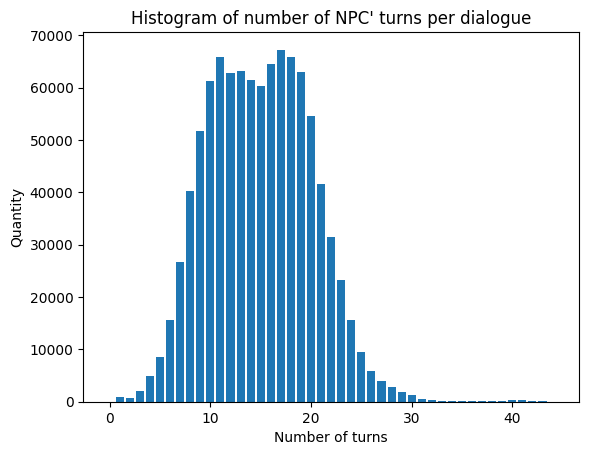
\includegraphics[width=.8\linewidth]{npc-turns-hist}
            \caption{Распределение частоты диалоговых ходов NPC по длине}\label{fig:npc-turns-hist}
      \end{minipage}\hfill
      \begin{minipage}{0.48\textwidth}
            \centering
            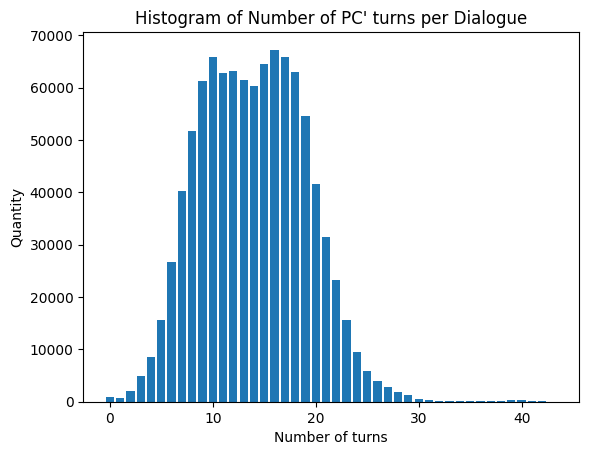
\includegraphics[width=.8\linewidth]{pc-turns-hist}
            \caption{Распределение частоты диалоговых ходов игрока по длине}\label{fig:pc-turns-hist}
      \end{minipage}
\end{figure}

\begin{figure}[H]
      \centering
      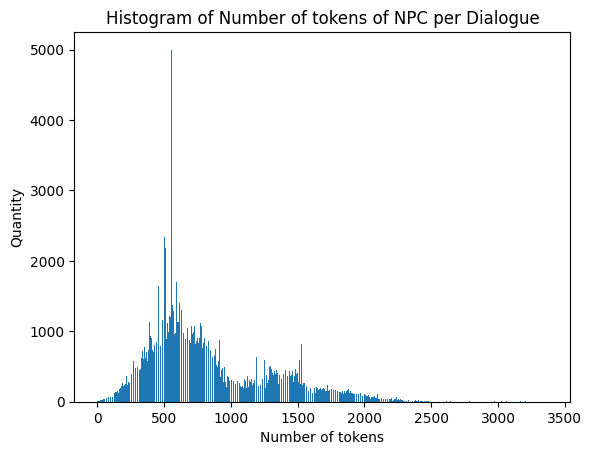
\includegraphics[width=0.5\textwidth]{npc-tokens-hist}
      \caption{Распределение частоты количества токенов в диалоге NPC по количеству}
      \label{fig:npc-tokens-hist}
\end{figure}

\begin{figure}[H]
      \centering
      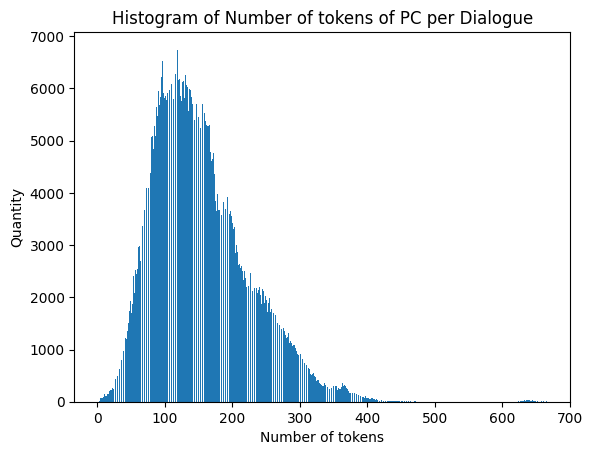
\includegraphics[width=0.5\textwidth]{pc-tokens-hist}
      \caption{Распределение частоты количества токенов в диалоге игрока по количеству}
      \label{fig:pc-tokens-hist}
\end{figure}

\section{ПОДГОТОВКА НАБОРА ДАННЫХ DNDD ДЛЯ ОБУЧЕНИЯ МОДЕЛЕЙ}

После фазы сбора диалоговых данных и генерации параметров NPC, включающих в себя идентификаторы, характеристики, мировозрение, мотивацию и слабости, следующим логическим этапом становится подготовка собранных данных к процессу обучения модели. Этот процесс включает в себя конкатенацию данных в строковом формате.

\subsection{ЭМУЛЯЦИЯ ДИАЛОГОВЫХ ВЗАИМОДЕЙСТВИЙ}

Особое внимание следует уделить диалоговым взаимодействиям между NPC и игроком. В контексте набора данных, где хранятся полные версии диалогов, эмуляция процесса общения игрока с NPC требует разбиения истории диалога на подмножества. В этом случае диалог представляет собой серию ходов между игроком и NPC, и основной задачей модели является продолжение данного диалога, т.е. совершение следующего хода в диалоге.

При таком подходе модель обучается на основе итеративного процесса диалога, что способствует приближению к более реалистичному моделированию процесса диалога. Это позволяет на каждом этапе оптимизировать процесс обучения для достижения максимально эффективного результата.

\subsection{СТРУКТУРИРОВАНИЕ ВХОДНЫХ ДАННЫХ ДЛЯ ОБУЧЕНИЯ}

Для оптимизации процесса обучения, входная последовательность, а именно описание неигрового персонажа, история диалогов с игроком, последняя реплика игрока и реплика, которую должна сгенерировать модель, была разделена на сегменты, каждый из которых был помечен соответствующим образом. Такой подход к структурированию входных данных для модели позволяет ясно разделять различные компоненты входных данных, что облегчает задачу модели и способствует более эффективному обучению.

Для обозначения начала диалога используется уникальный идентификатор <<EMPTY>>, который функционирует как сигнал о том, что диалог только что был инициирован. В силу специфики набора данных DNDD, полученного из игр, где неигровые персонажи всегда начинают диалог первыми, было определено, что первая реплика игрока служит активацией диалога, и обозначена она идентификатором <<START DIALOGUE>>. В ходе последующего диалога реплики участников регистрируются в истории диалога с пометками <<Player: >> и <<NPC: >>, в зависимости от того, кто в данный момент выступает в роли говорящего.

\subsection{ОПТИМИЗАЦИЯ ДАННЫХ ПОД ПОТРЕБИТЕЛЬСКОЕ ОБОРУДОВАНИЕ}

Учитывая ограниченные вычислительные ресурсы потребительского уровня, включая оперативную память объемом 32 Гб и графическую карту NVIDIA GeForce RTX 3090 Ti с 24 Гб памяти, было необходимо ввести определенные ограничения на обрабатываемую историю диалогов. При превышении диалогом лимита в 1024 токенов, для обеспечения управляемости данных самые старые записи в диалоге подлежали удалению. Это позволяло оптимизировать использование доступных вычислительных ресурсов и обеспечивать стабильный процесс обучения моделей. 

Также было ограничено максимальное количество диалогов, которых может иметь игрок с одним неигровым персонажем. Этот подход позволяет получить более разнообразный набор данных с уменьшенным размером выборки.

Итоговые данные выглядят следующим образом.
Входная последовательность:
\texttt{\\Below is the definition of in-game NPC.\\
      NPC Name: Digby\\
      Alignment: Neutral\\
      Description: A burly, bearded man with a thick accent and a penchant for trapping.\\
      Personality traits: Digby is a bit of a glutton, and often overindulges in food and drink.\\
      Flaws: Digby is motivated by the prospect of making a profit from his trapping.\\
      Motivation: Digby is a gruff, no-nonsense man who is quick to anger and slow to trust. He is a hard worker and is not afraid to get his hands dirty. He is also a bit of a glutton, and often overindulges in food and drink.\\
      Dialogue history:\\
      Player: START DIALOGUE\\
      NPC: *burp* Think I had too much to drink last night. Heh! What am I sayin'?! There's no such thing, says my brothers. Hey, who are you, anyway?\\\\
      Player query: Who are you?\\
      Respond to player's query based on defined NPC:\\}

Ожидаемый ответ: \texttt{I'm Digby. I'm a trapper 'round these parts. Me and my brothers catch all sorts of varmints, skin 'em, and sell 'em. Course, it's hard lately now that Emmerich is pokin' 'round.}

Детальная реализация обработки набора данных c документацией доступна в приложении \ref{app:code}.